\documentclass[aspectratio=169, 11pt]{beamer}
\usetheme{metropolis}

\usepackage{graphicx}
\usepackage{booktabs}
\usepackage{xcolor}
\usepackage{appendixnumberbeamer}

% Custom colors
\definecolor{alertred}{RGB}{204, 36, 29}
\definecolor{okgreen}{RGB}{40, 140, 40}
\definecolor{noteblue}{RGB}{30, 90, 160}

\setbeamercolor{alerted text}{fg=alertred}

\graphicspath{{figs/}}

\title{v14 Natural Gas Model:\\Dual Value Investigation}
\subtitle{Root Cause Analysis and Remaining Issues}
\author{Caleb Sy}
\date{March 2026}
\institute{PhD Research Briefing}

\begin{document}

\maketitle

%% ============================================================
%% PART I: BACKGROUND
%% ============================================================

\section{Background}

% ---- Slide 2: Model Overview ----
\begin{frame}{Model Overview}
  The v14 daily natural gas market model:
  \begin{itemize}
    \item \textbf{Scope}: 372 days (Dec 25 2018 -- Dec 31 2019), state-level nodes, U.S. pipelines
    \item \textbf{Method}: Linear program minimizing total system cost \\
      (production + transport + storage + slack penalties)
    \item \textbf{Two-part structure}:
      \begin{description}
        \item[Part 2] Base price solve --- production free to optimize; \\
          consumption reduced by $\max(0,\;\text{demand} - \text{supply})$
        \item[Part 3] Storage re-solve --- production fixed at historical; \\
          full consumption restored; storage withdrawal cost $\approx$ Part 2 dual $+$ rolling delta
      \end{description}
    \item \textbf{Output}: Nodal dual values $=$ shadow prices $=$ model gas prices
  \end{itemize}
\end{frame}

% ---- Slide 3: The Problem ----
\begin{frame}{The Problem: Part 3 Prices Are Implausibly Low}
  After implementing the Part 3 storage re-solve:
  \begin{itemize}
    \item Part 3 nodal duals \alert{systematically fall below} Part 2 on many days
    \item 15 ``drop days'' show extreme collapses: TX drops from \$2.50 $\to$ \$0.01
    \item Drops are concentrated in \textbf{injection season} (spring/summer, days 76--260)
    \item Broader pattern: P3 $<$ P2 on \textbf{245 of 372 days} across producing nodes
  \end{itemize}
  \vspace{0.3em}
  \alert{Two distinct problems emerged:}
  \begin{enumerate}
    \item \textbf{Producing node drops} (TX, PA, LA, CO) --- root cause found, fix implemented
    \item \textbf{NE demand node depression} (MA, CT, RI, NH, ME) --- pipeline congestion, under investigation
  \end{enumerate}
\end{frame}

%% ============================================================
%% PART II: DUAL DROP INVESTIGATION
%% ============================================================

\section{Investigation 1: Producing Node Dual Drops}

% ---- Slide 4: Symptom ----
\begin{frame}{Symptom: Production Constraint Drives Dual Depression}
  \begin{figure}
    \centering
    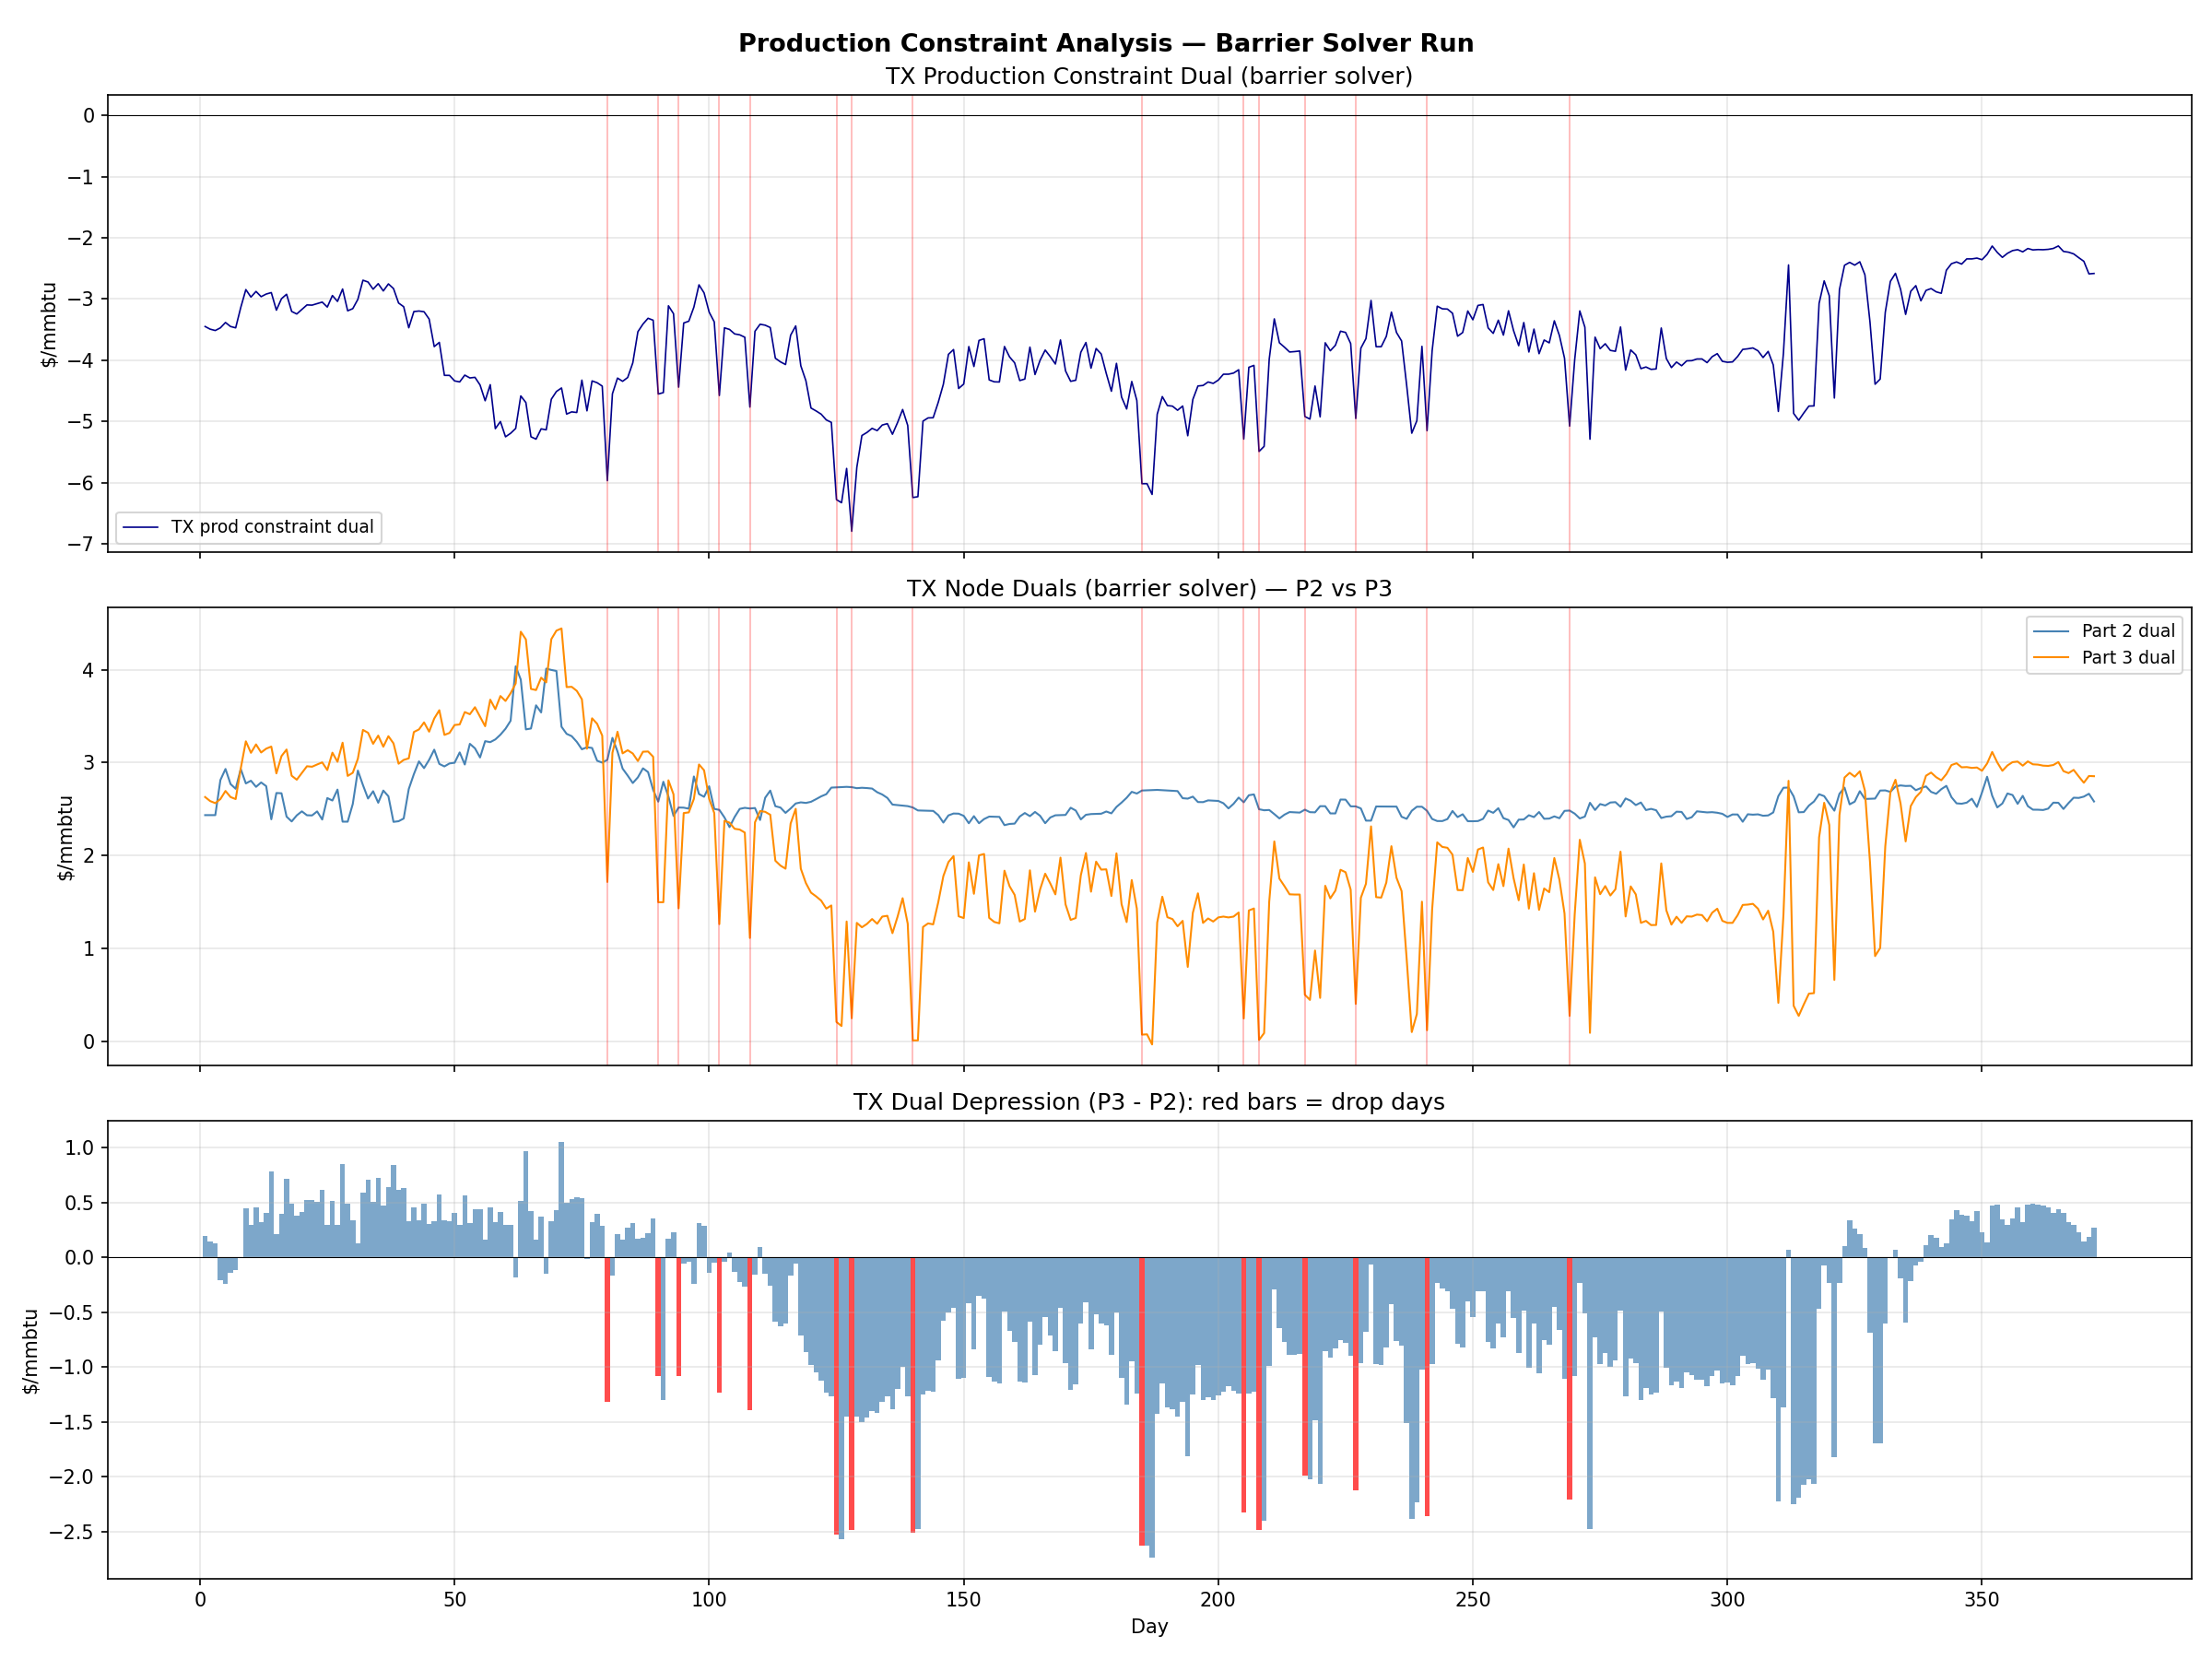
\includegraphics[width=0.92\linewidth]{07_prod_constraint_dual_timeseries.png}
  \end{figure}
  \vspace{-0.5em}
  {\small \textbf{Top}: TX production constraint dual (always negative --- model wants to produce \emph{less}).
  \textbf{Mid}: P2 vs P3 nodal duals. \textbf{Bottom}: P3$-$P2 gap; red bars = drop days.}
\end{frame}

% ---- Slide 5: Hypothesis Test ----
\begin{frame}{Ruling Out LP Degeneracy}
  \textbf{Initial hypothesis}: Dual drops are LP degeneracy (non-unique shadow prices).
  \vspace{0.3em}

  \textbf{Test}: Solved Part 3 with 4 independent Gurobi algorithms:
  \begin{enumerate}
    \item Primal simplex
    \item Dual simplex
    \item Barrier + crossover
    \item Barrier only (no crossover)
  \end{enumerate}
  \vspace{0.3em}

  \textbf{Result}: All 4 methods produce \alert{identical duals to machine precision} on every day.
  \vspace{0.3em}

  \begin{block}{Conclusion}
    Duals are \textbf{unique} $\Rightarrow$ \textbf{not degeneracy}. The low prices are the \emph{correct} economic signal of a structural oversupply forced by a model constraint.
  \end{block}
\end{frame}

% ---- Slide 6: Root Cause ----
\begin{frame}{Root Cause: Forced Overproduction}
  \textbf{The constraint}: In Part 3, \texttt{Qstep\_prod} is an \alert{equality} ($=$), forcing total production at each node to match historical \texttt{NA\_production} exactly.

  \vspace{0.5em}
  \textbf{The mechanism}:
  \begin{itemize}
    \item Part 2 freely optimizes production $\to$ produces $\sim$0.2\% below historical
    \item Part 3 forces production back up to historical $\to$ creates excess supply
    \item During injection season, excess has nowhere to go:
      \begin{itemize}
        \item Injection capped by \texttt{TotalDailyInjection} equality
        \item Withdrawals = 0 in injection season
        \item All slacks = 0
      \end{itemize}
  \end{itemize}
  \vspace{0.3em}

  \textbf{Evidence}: Production constraint dual averages \alert{$-$\$3.84/mmbtu} at TX. \\
  Correlation with dual depression: $r = 0.70$ (TX), $r = 0.98$ (PA, LA, CO).
\end{frame}

% ---- Slide 7: The Fix ----
\begin{frame}{The Fix: One Character Change}
  \begin{figure}
    \centering
    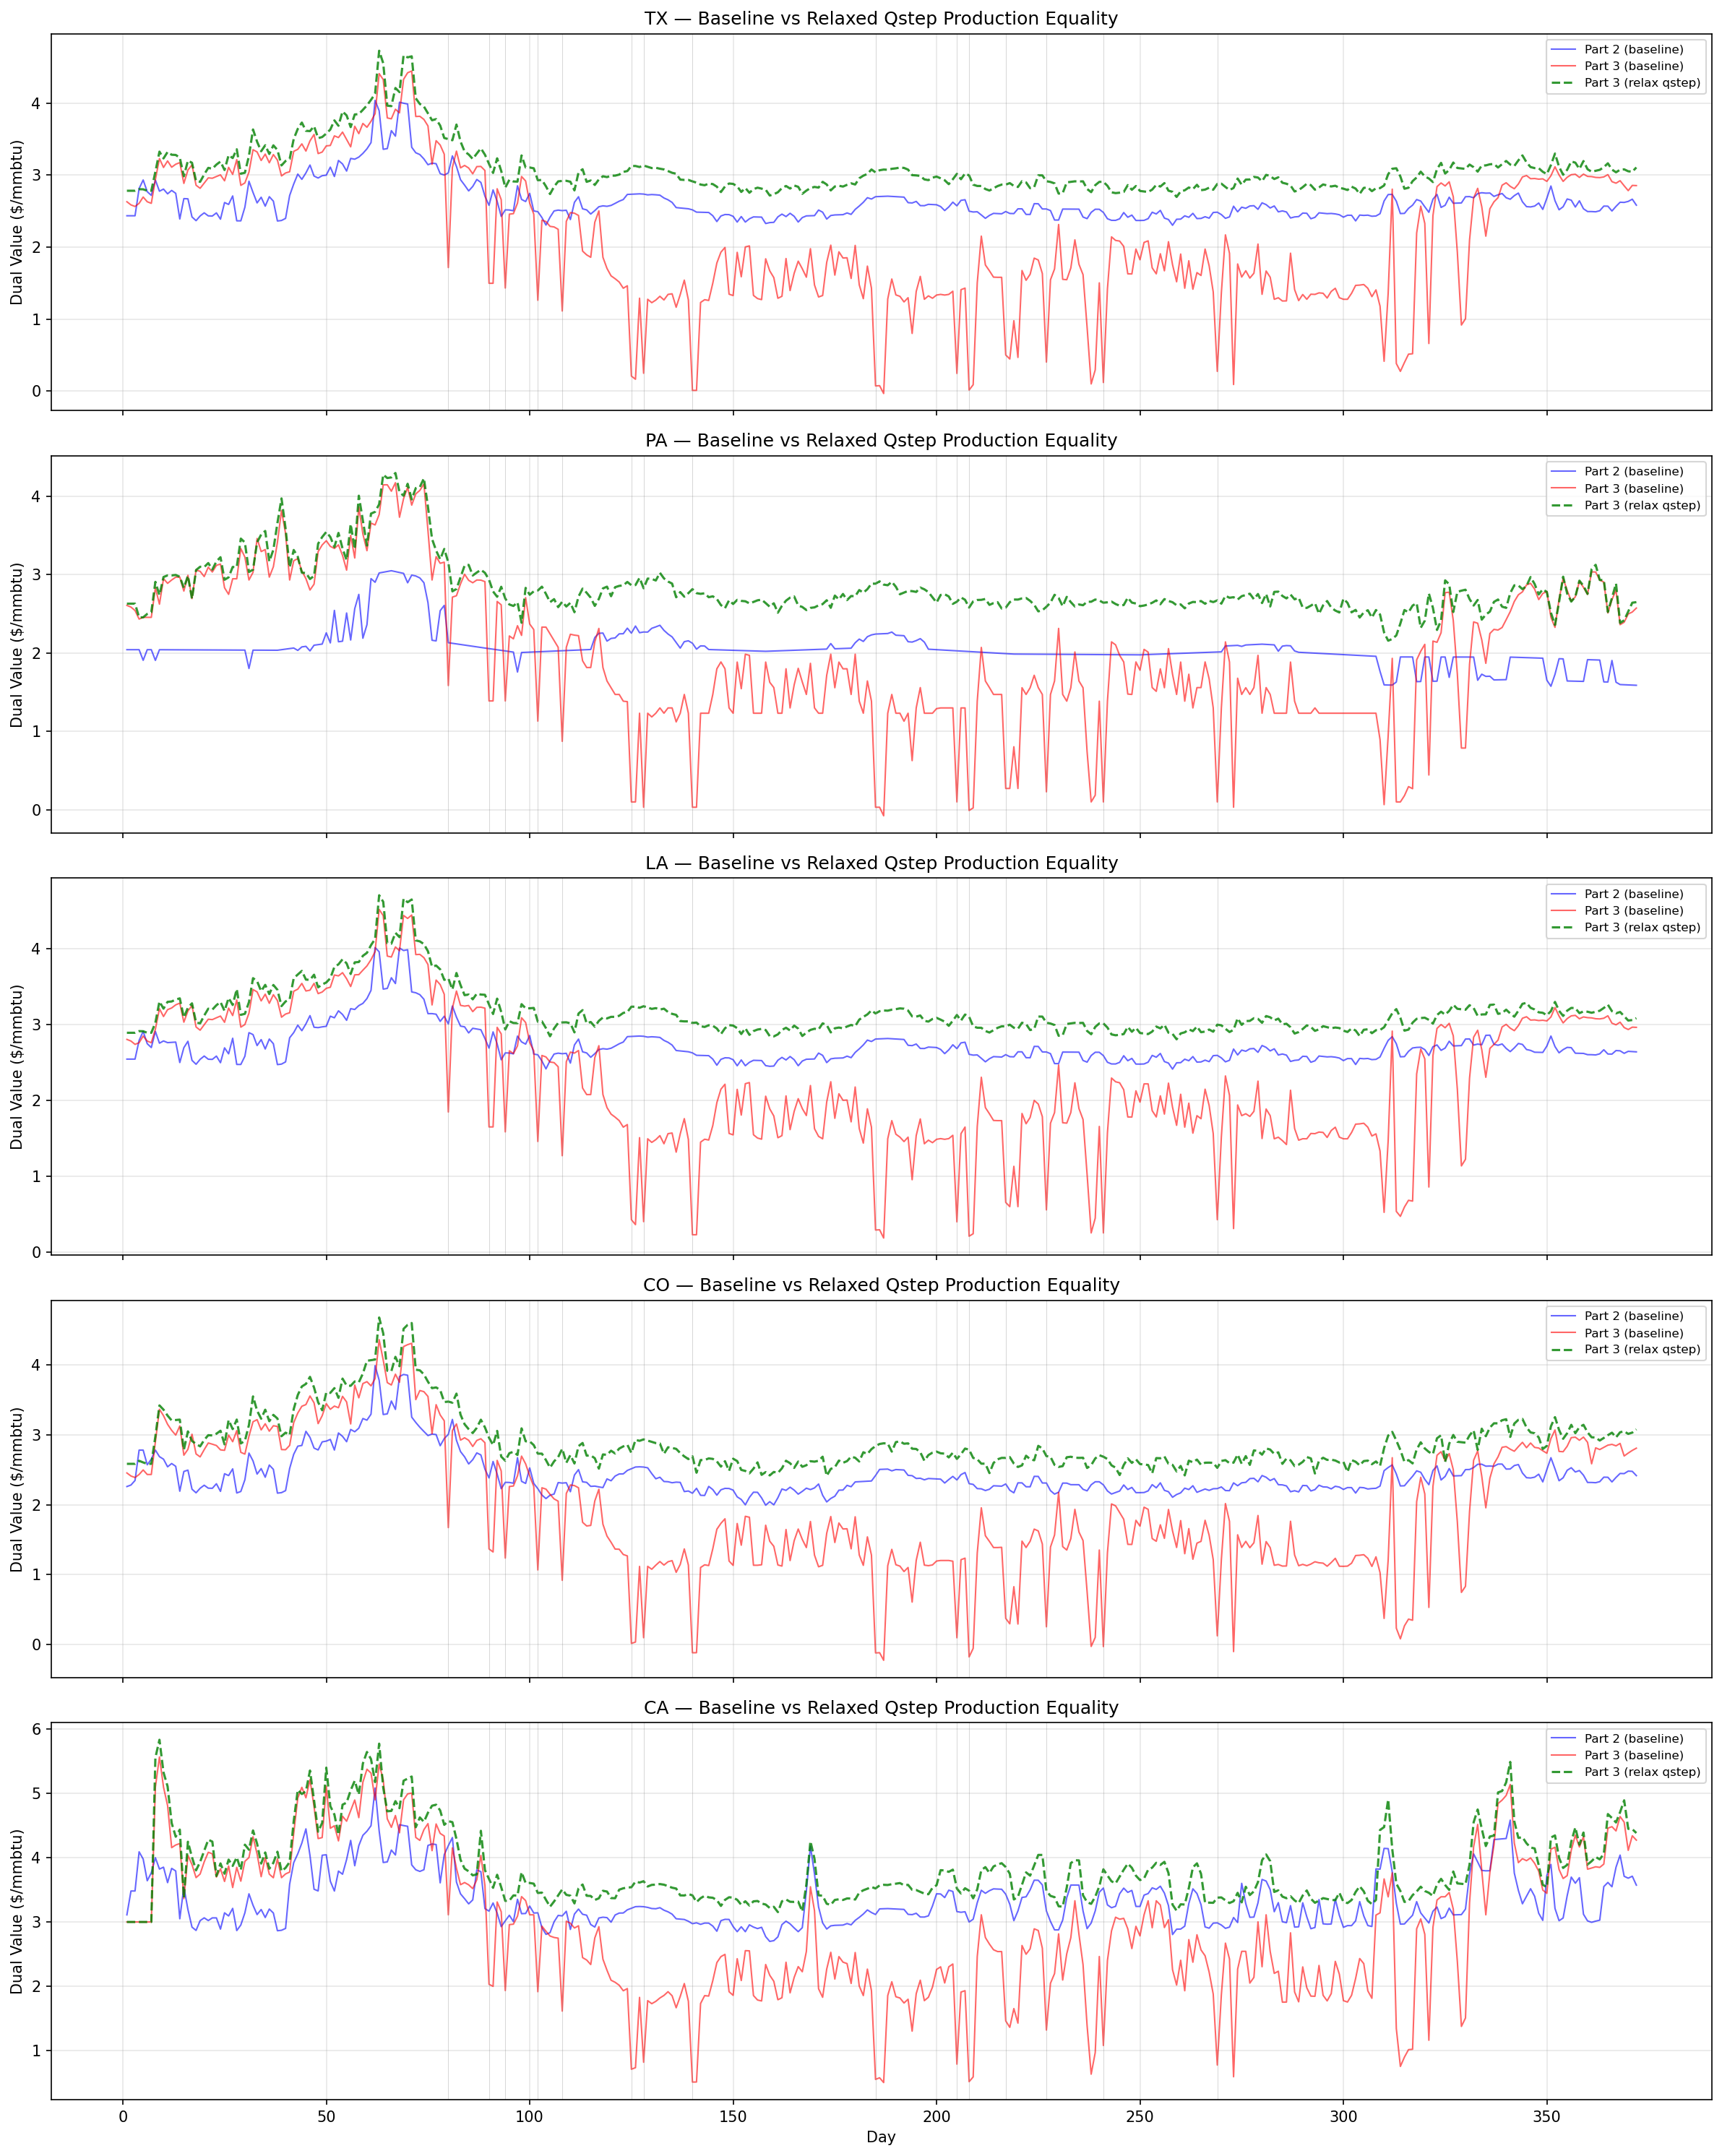
\includegraphics[width=0.78\linewidth]{09b_relax_qstep_comparison.png}
  \end{figure}
  \vspace{-0.5em}
  {\small \texttt{Qstep\_prod}: \texttt{==} $\to$ \texttt{<=} (line 368 of \texttt{v14\_gas\_model\_dev.py}).
  \textcolor{red}{Red} = P2, \textcolor{blue}{Blue} = P3 baseline, \textcolor{green!60!black}{Green dashed} = P3 relaxed.
  P3 now tracks P2 at all 5 producing nodes.}
\end{frame}

% ---- Slide 8: Verification ----
\begin{frame}{Verification: Before vs.\ After}
  \begin{table}
    \centering
    \begin{tabular}{lcc}
      \toprule
      \textbf{Metric} & \textbf{Before} (\texttt{==}) & \textbf{After} (\texttt{<=}) \\
      \midrule
      Days with TX dual $< \$1.00$    & 31            & \textcolor{okgreen}{\textbf{0}} \\
      Minimum TX dual                 & $-$\$0.03     & \textcolor{okgreen}{\textbf{\$2.70}} \\
      Mean P3$-$P2 gap                & $-$\$0.45     & \textcolor{okgreen}{\textbf{+\$0.45}} \\
      Prod constraint dual (mean)     & $-$\$5.36     & \textcolor{okgreen}{\textbf{\$0.00}} \\
      Production change               & ---           & \textbf{0.0\%} \\
      Pipeline flow change            & ---           & 24.8\% \\
      Storage injection change        & ---           & 35.4\% \\
      \bottomrule
    \end{tabular}
  \end{table}
  \vspace{0.5em}

  \begin{itemize}
    \item Supply curves still incentivize the same production $\to$ \textbf{0\% production change}
    \item Dispatch pattern adjusts (flows, injection redistribute) --- expected and correct
    \item Prod constraint dual $= 0$ on all days $\to$ constraint no longer binding
  \end{itemize}
\end{frame}

%% ============================================================
%% PART III: NE INJECTION SEASON
%% ============================================================

\section{Investigation 2: New England Injection Season}

% ---- Slide 9: Remaining Problem ----
\begin{frame}{Remaining Problem: NE Nodes Still Depressed}
  \begin{figure}
    \centering
    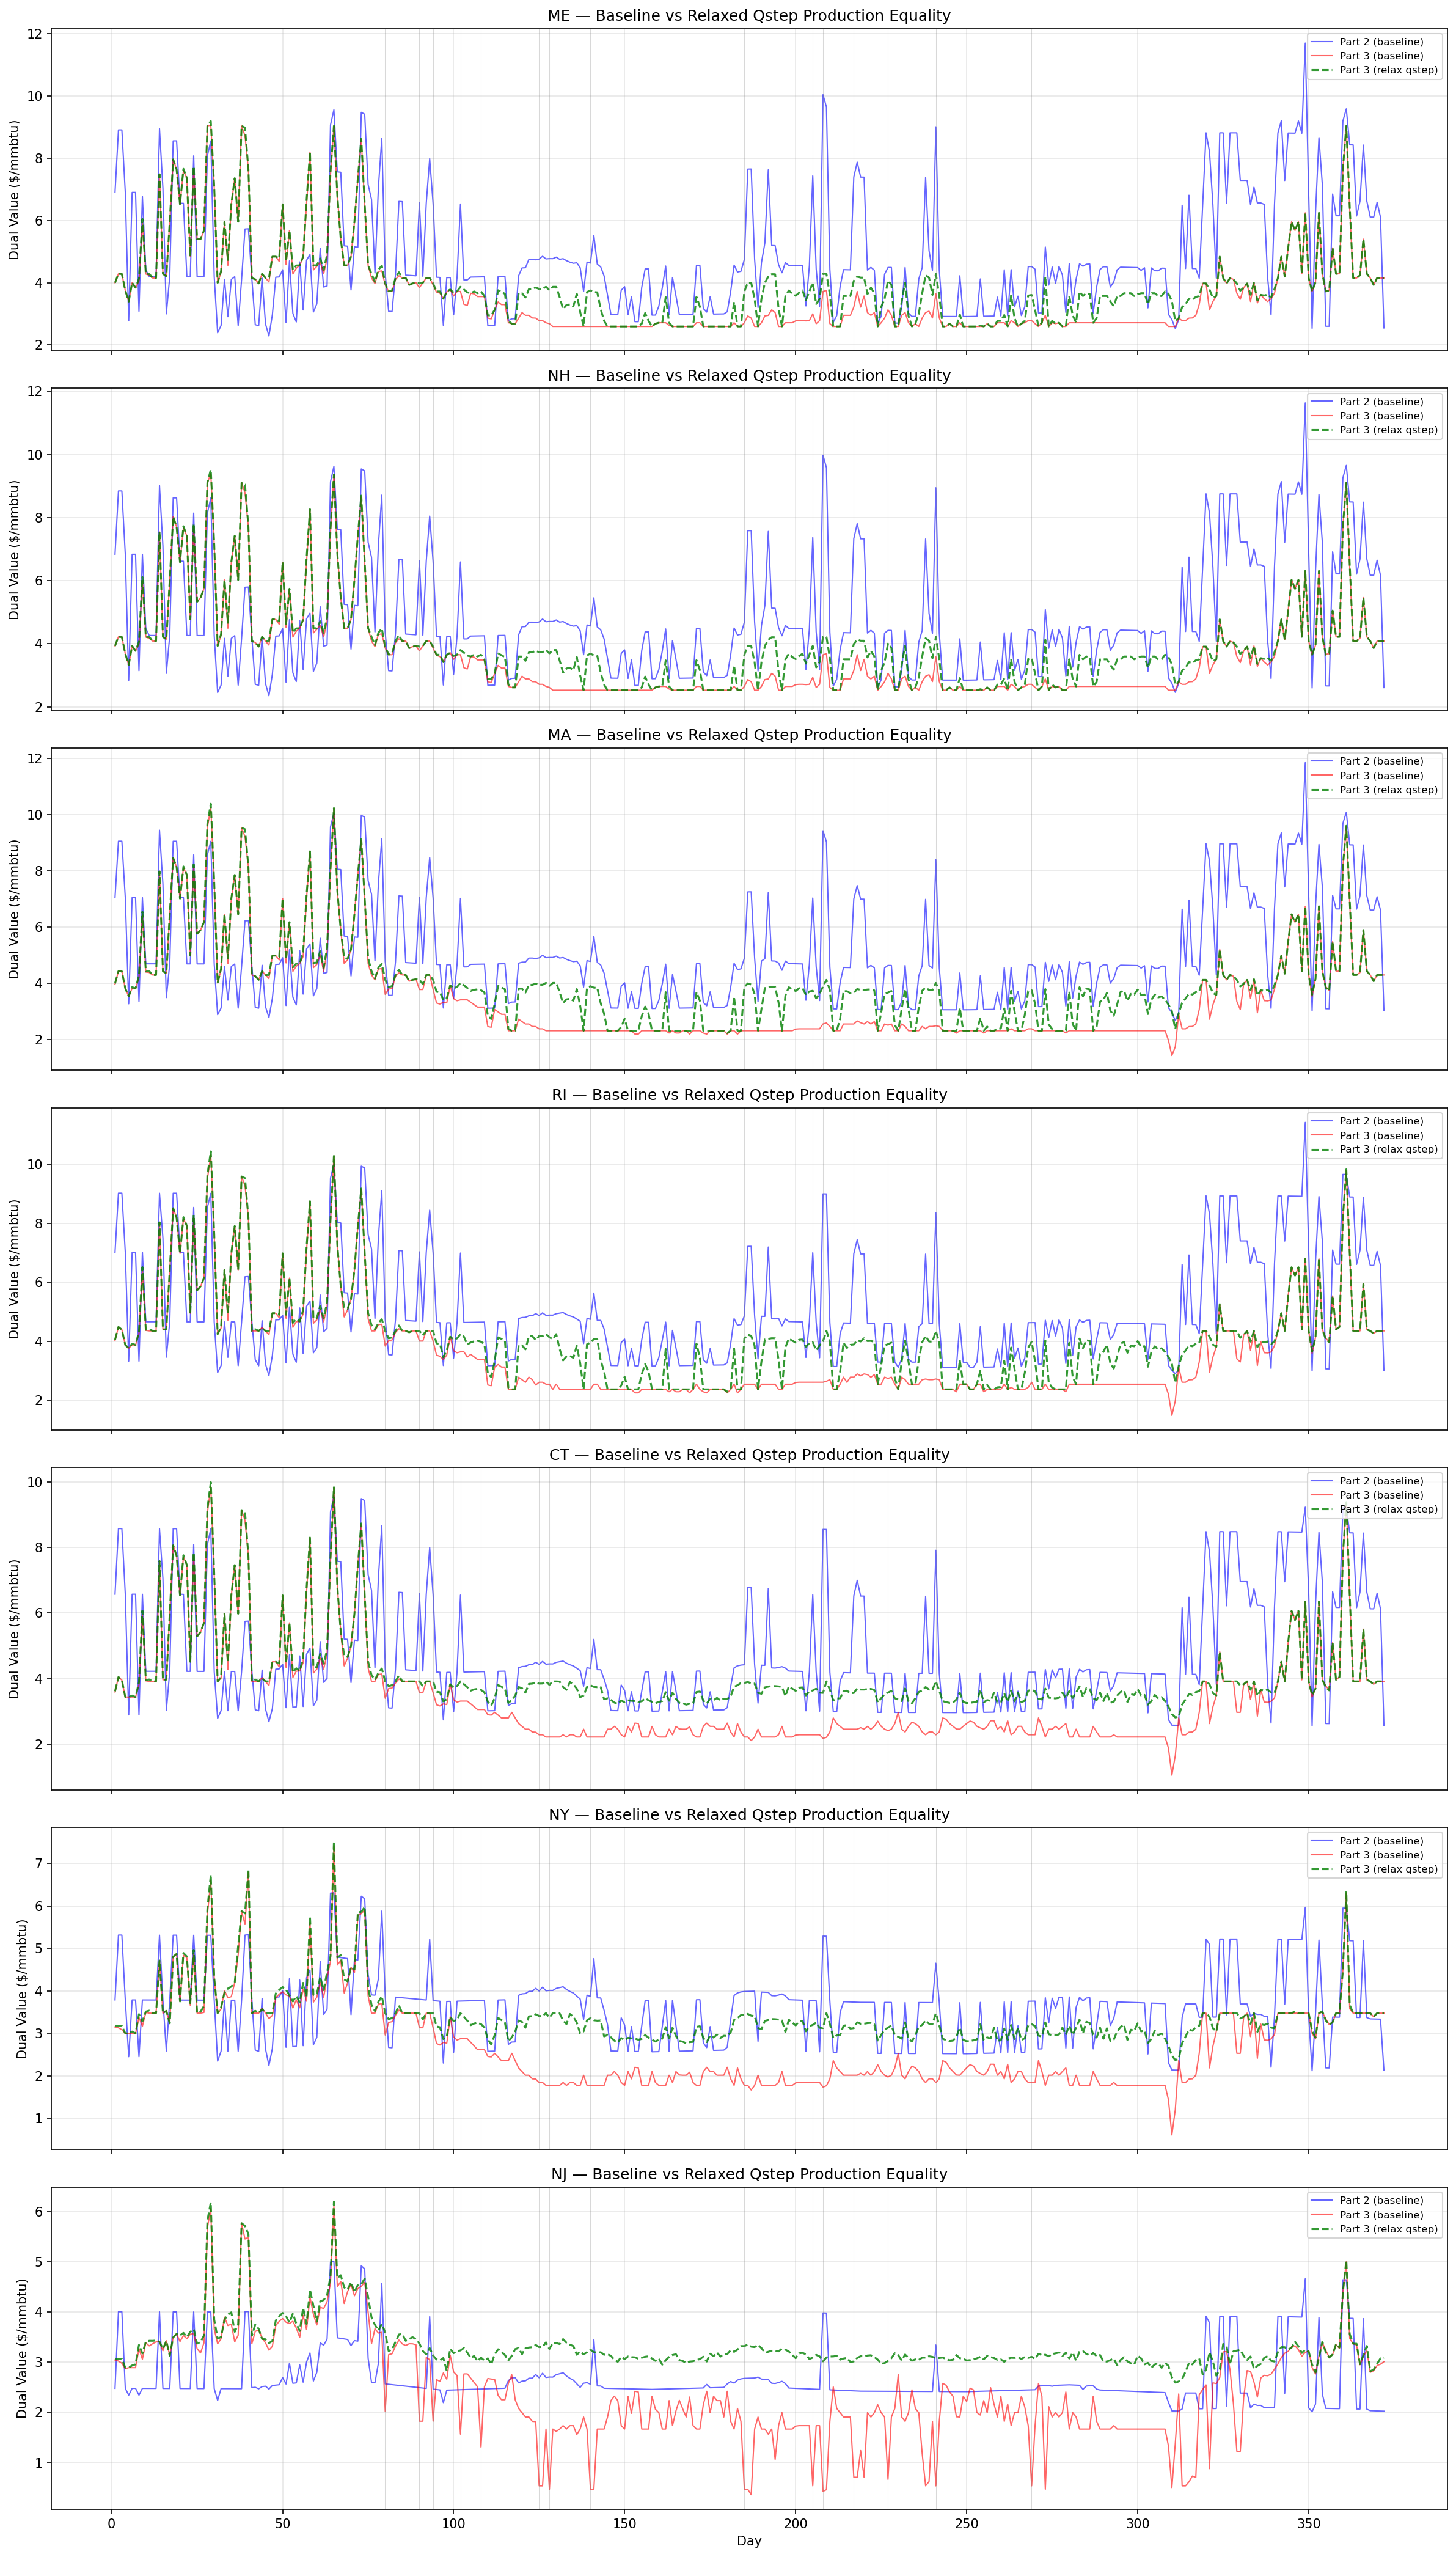
\includegraphics[width=0.78\linewidth]{09b_relax_qstep_comparison_new_england.png}
  \end{figure}
  \vspace{-0.5em}
  {\small Even with the \texttt{Qstep\_prod} fix, NE states (ME, NH, MA, RI, CT, NY, NJ) show
  P3 duals \alert{well below P2} during injection season. This is a separate mechanism.}
\end{frame}

% ---- Slide 10: Price Gradient ----
\begin{frame}{Price Gradient Along the Supply Chain}
  \begin{figure}
    \centering
    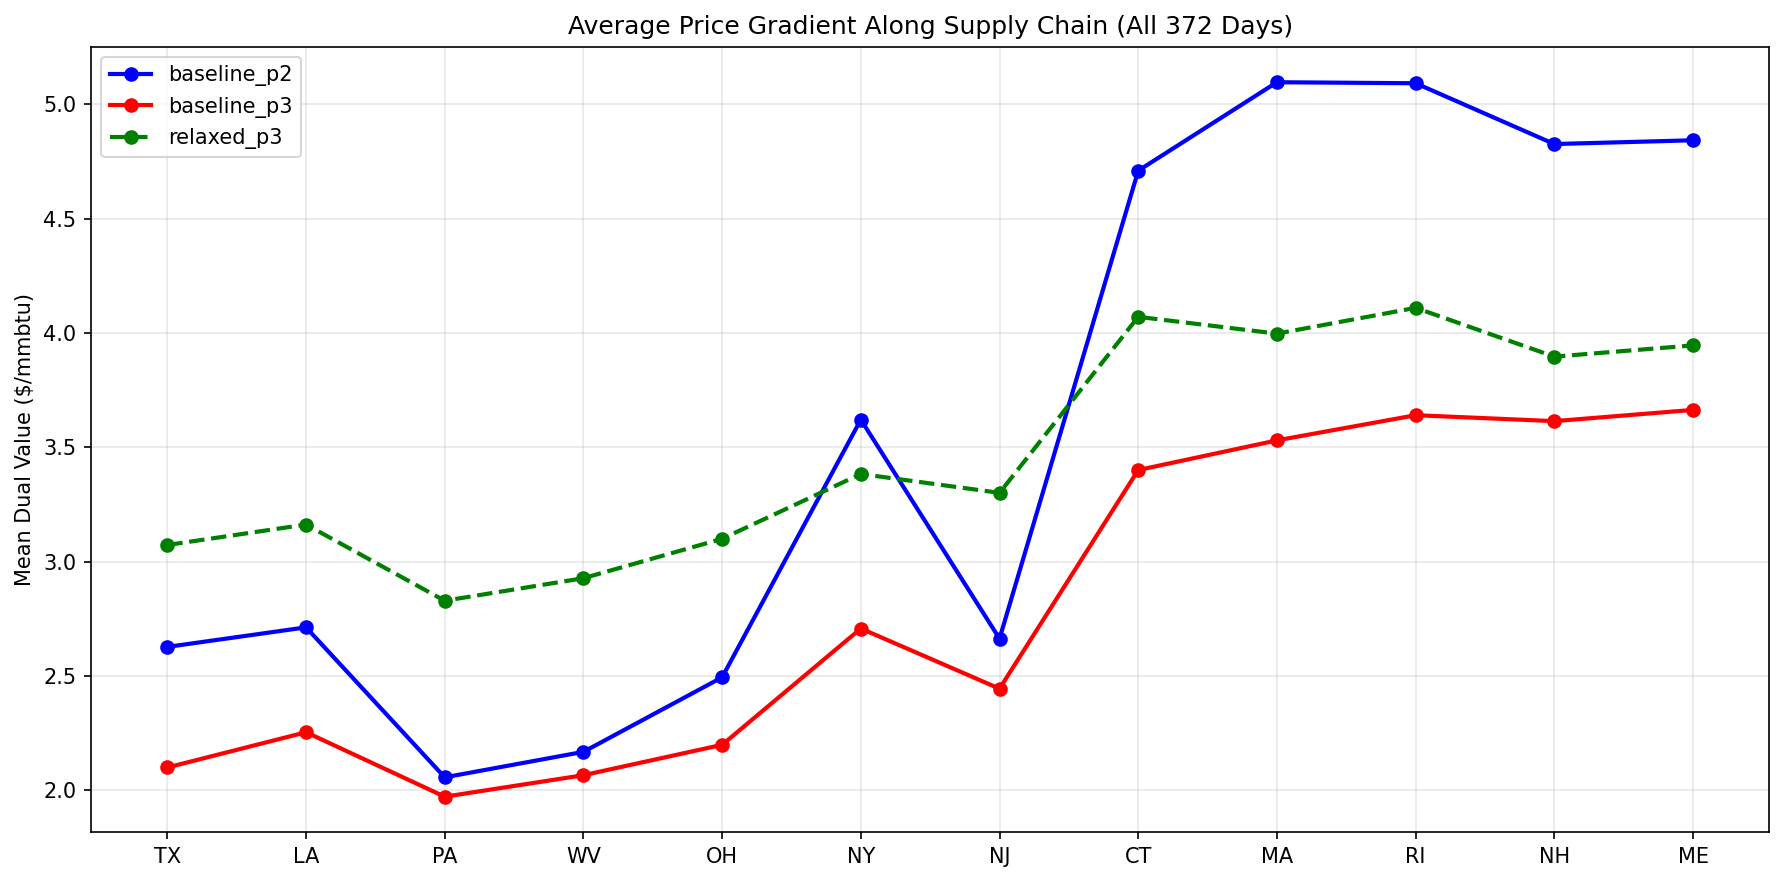
\includegraphics[width=0.88\linewidth]{03_avg_price_gradient.png}
  \end{figure}
  \vspace{-0.5em}
  {\small Mean dual by node, ordered from producing (TX) to consuming (ME) regions.
  \textcolor{blue}{\textbf{Blue}} = P2, \textcolor{red}{\textbf{Red}} = P3 baseline, \textcolor{green!60!black}{\textbf{Green}} = P3 relaxed.
  The relaxed P3 (green) closes the gap at producing nodes but \alert{still diverges sharply from P2 in NE}.}
\end{frame}

% ---- Slide 11: Pipeline Congestion ----
\begin{frame}{Root Cause 1: Pipeline Congestion}
  Part 3 restores full consumption (+8.6\% vs.\ Part 2), but NE pipelines are already at capacity.

  \vspace{0.5em}
  \textbf{Key findings}:
  \begin{itemize}
    \item \textbf{30 pipeline segments} permanently at capacity in Part 3
    \item PA $\to$ NY pipeline at \alert{100\% utilization on all 372 days}
    \item NE core entry lines (into CT, MA, RI, NH, ME) saturated during injection season
    \item Part 3 adds $\sim$8.6\% more demand through the same constrained pipelines
  \end{itemize}

  \vspace{0.5em}
  \begin{block}{Effect}
    Congested pipelines create a \textbf{price cliff} between NY/NJ and NE core states. Higher demand cannot be met $\to$ marginal gas value drops (floor price emerges).
  \end{block}
\end{frame}

% ---- Slide 12: Flow Reversal ----
\begin{frame}{Flow Reversal: MA Flips from Importer to Exporter}
  \begin{figure}
    \centering
    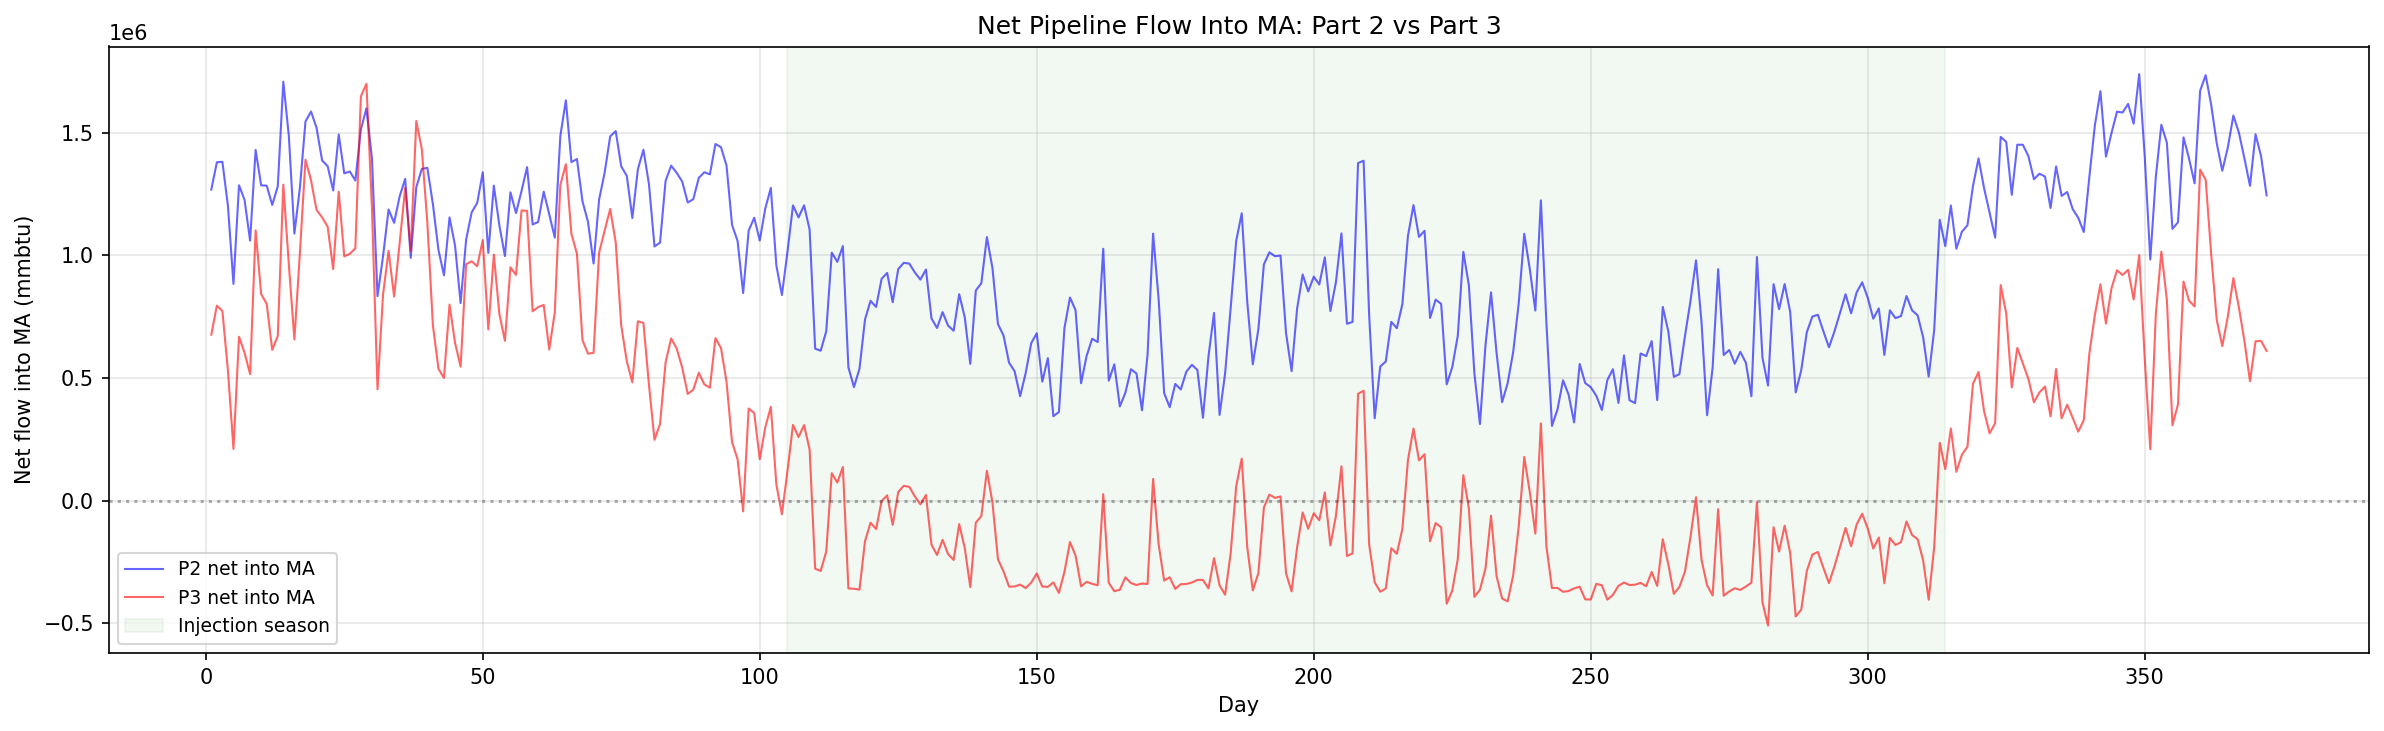
\includegraphics[width=0.92\linewidth]{07_ma_net_inbound.png}
  \end{figure}
  \vspace{-0.5em}
  {\small Net pipeline flow into Massachusetts. \textcolor{blue}{\textbf{Blue}} = Part 2 (always positive = importer). \textcolor{red}{\textbf{Red}} = Part 3 (frequently negative in injection season = \alert{MA becomes an exporter}).
  The \textcolor{green!30!black}{green shading} marks the injection season.}
\end{frame}

% ---- Slide 13: Injection Drain ----
\begin{frame}{Root Cause 2: NY Storage Injection Drains NE Inflow}
  \begin{figure}
    \centering
    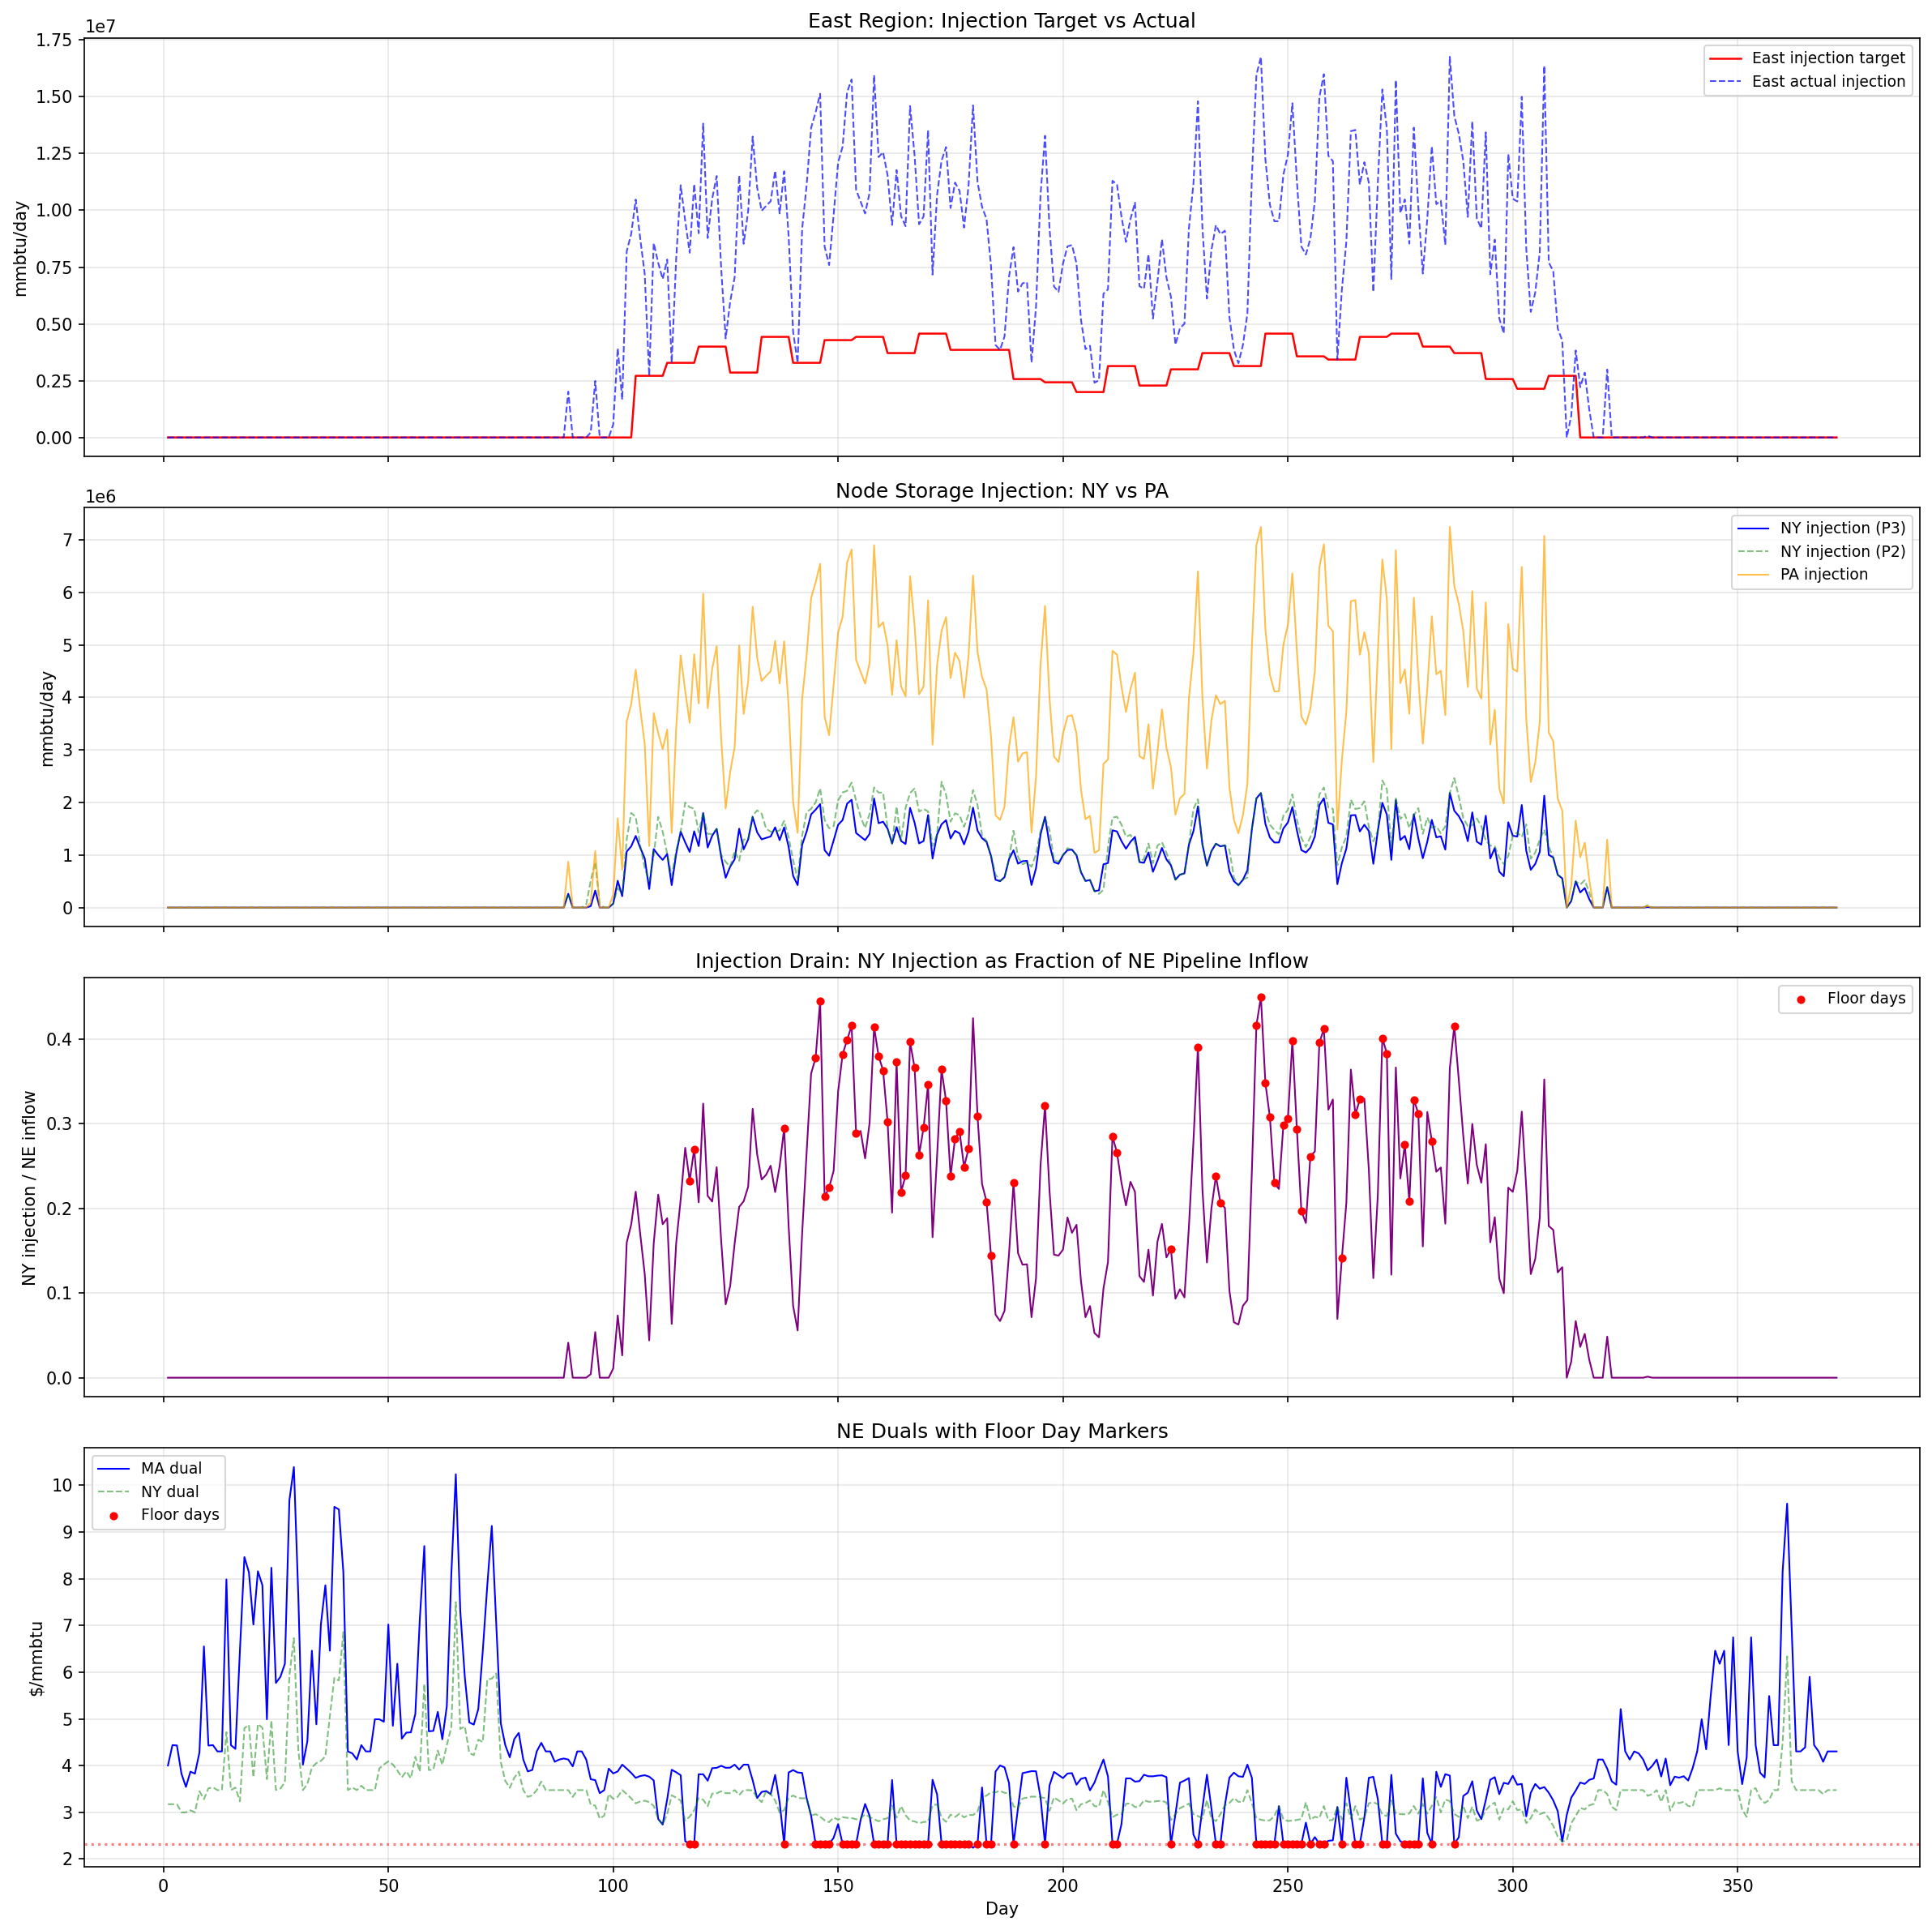
\includegraphics[width=0.68\linewidth]{08_injection_drain.png}
  \end{figure}
  \vspace{-0.5em}
  {\small \textbf{Panel 1}: East region injection far exceeds target. \textbf{Panel 2}: NY injection dominates.
  \textbf{Panel 3}: NY absorbs \alert{22.5\%} of NE pipeline inflow. Red dots = floor days.
  \textbf{Panel 4}: MA dual hits \$2.32 floor on floor days.}
\end{frame}

% ---- Slide 14: Storage Cost Volatility ----
\begin{frame}{Root Cause 3: Storage Withdrawal Cost Volatility}
  \begin{figure}
    \centering
    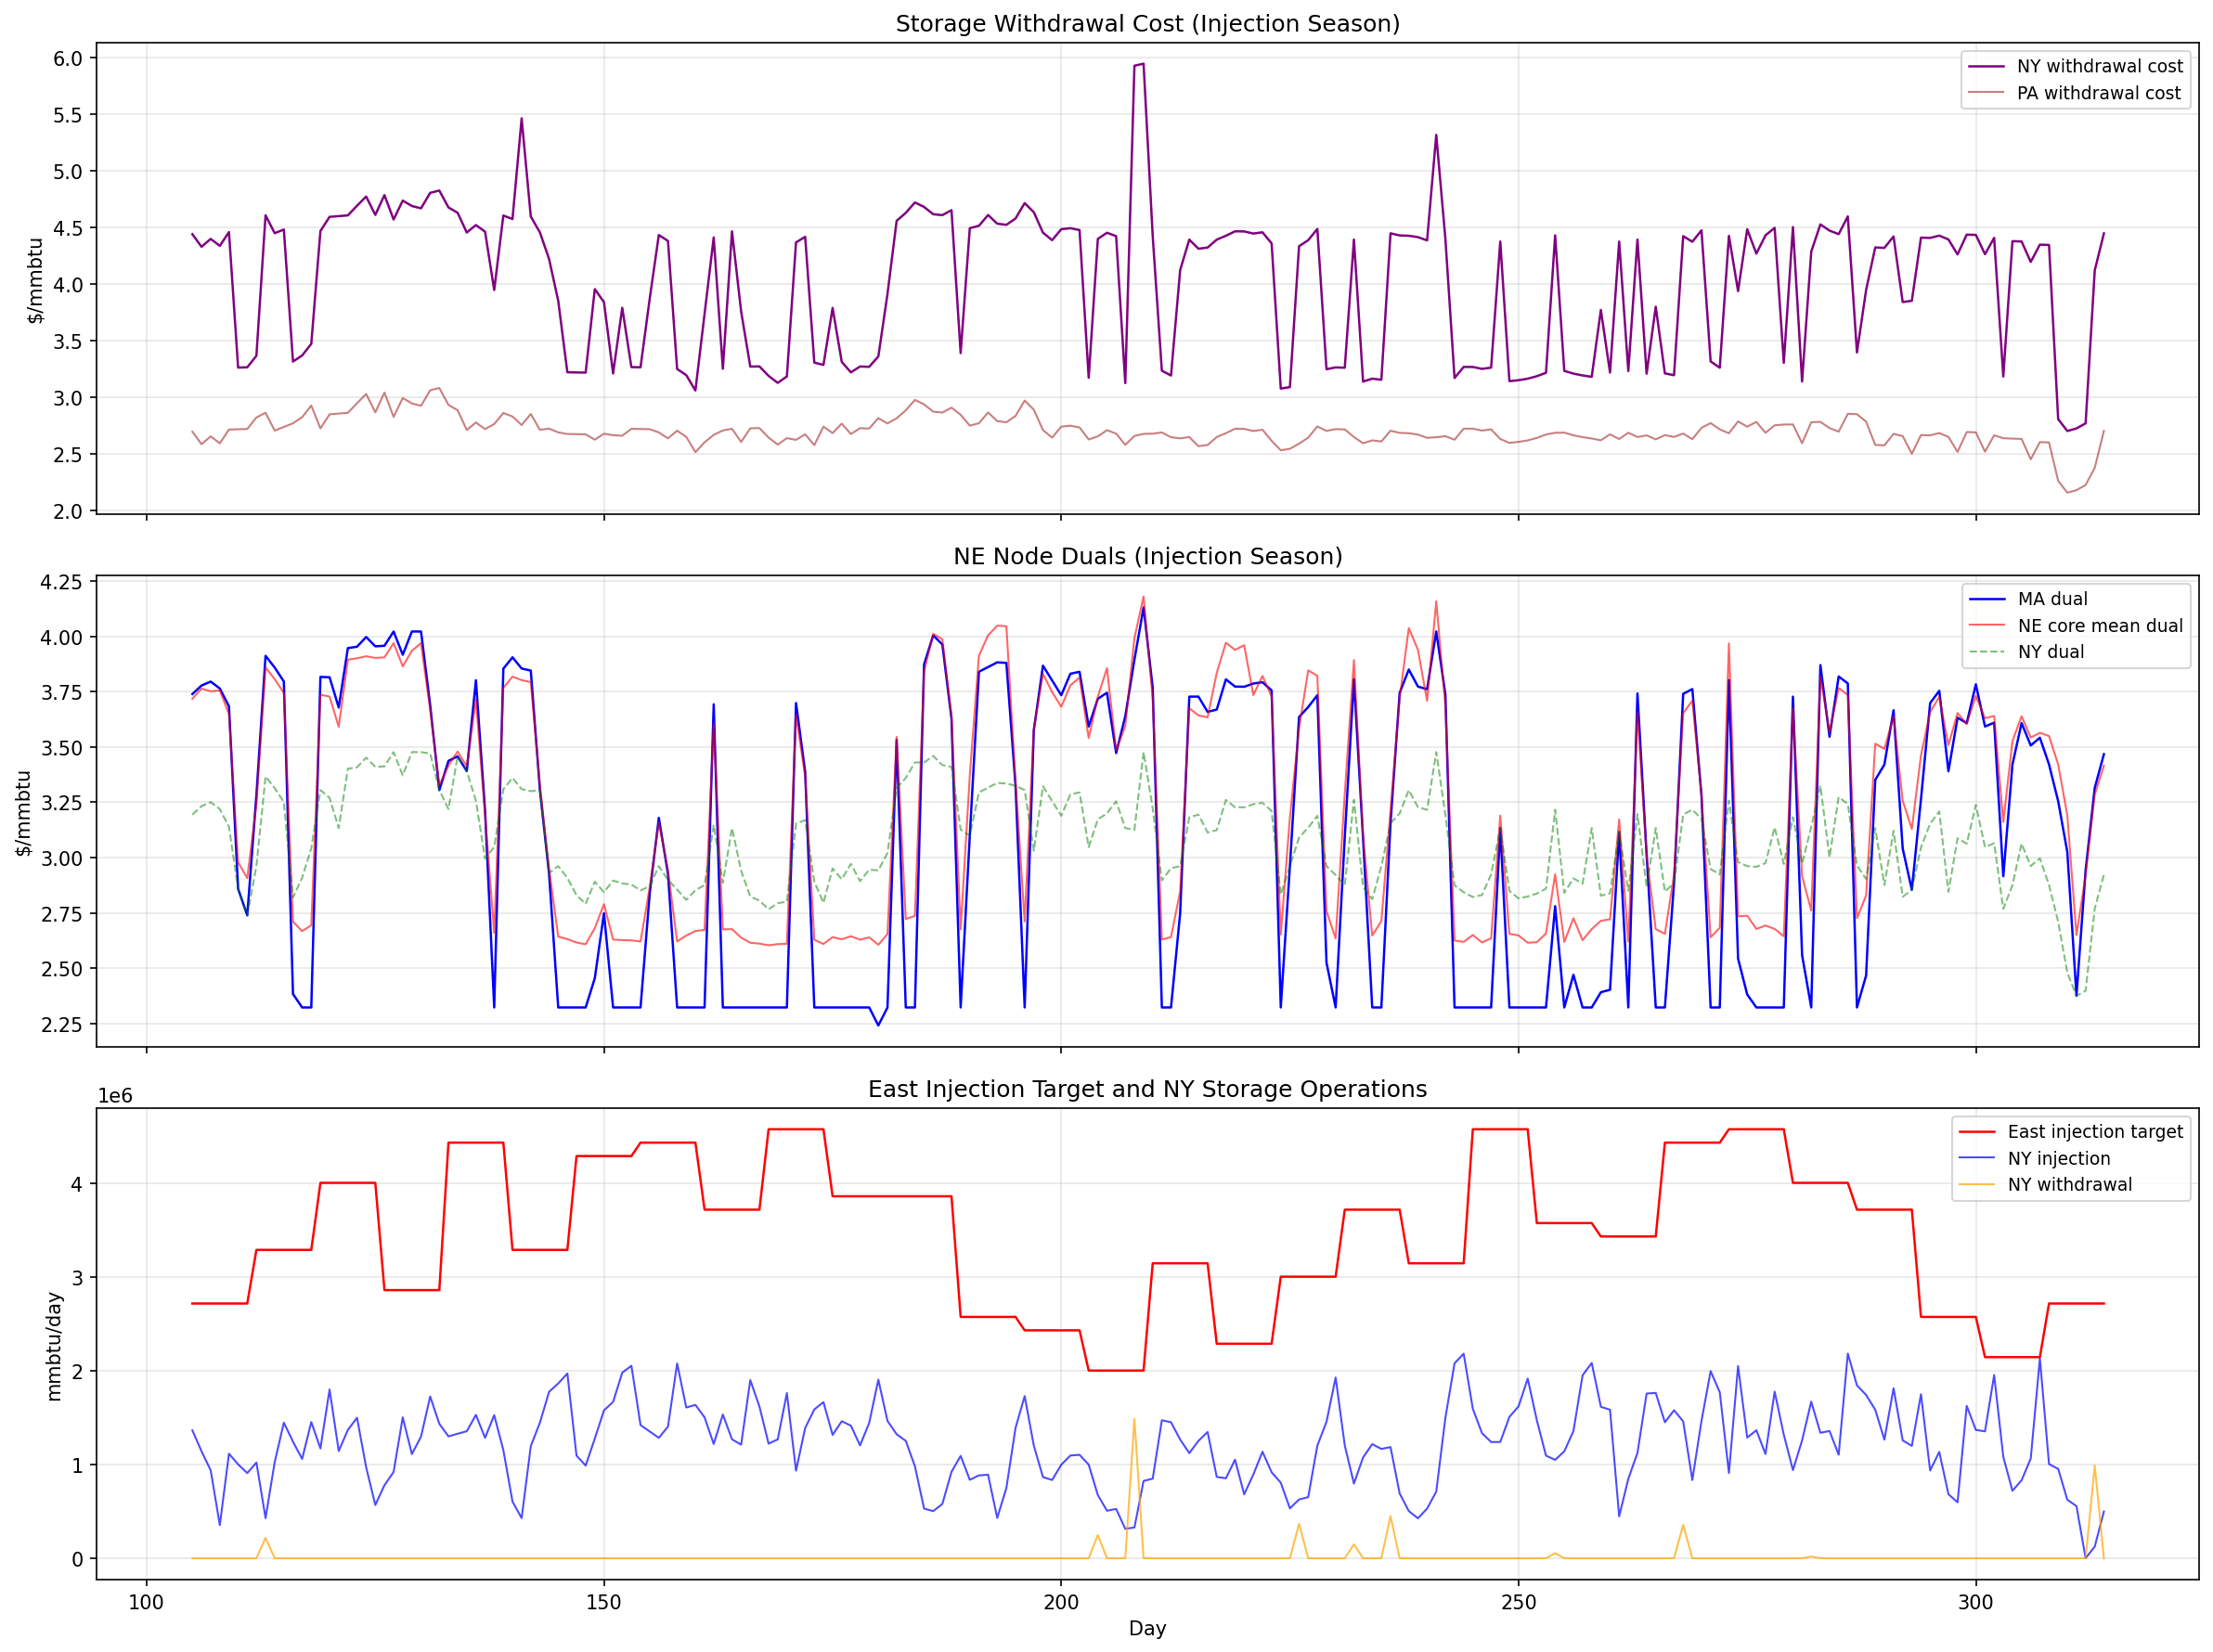
\includegraphics[width=0.82\linewidth]{06_storage_cost_volatility.png}
  \end{figure}
  \vspace{-0.5em}
  {\small \textbf{Top}: NY withdrawal cost swings $\pm$\$0.41/day (7-day rolling window artifact).
  \textbf{Mid}: NE duals oscillate in sync. \textbf{Bottom}: East injection target (step function from regional allocation). Correlation $r = 0.76$.}
\end{frame}

% ---- Slide 15: Cost vs Dual Scatter ----
\begin{frame}{Storage Cost Drives Dual Volatility}
  \begin{figure}
    \centering
    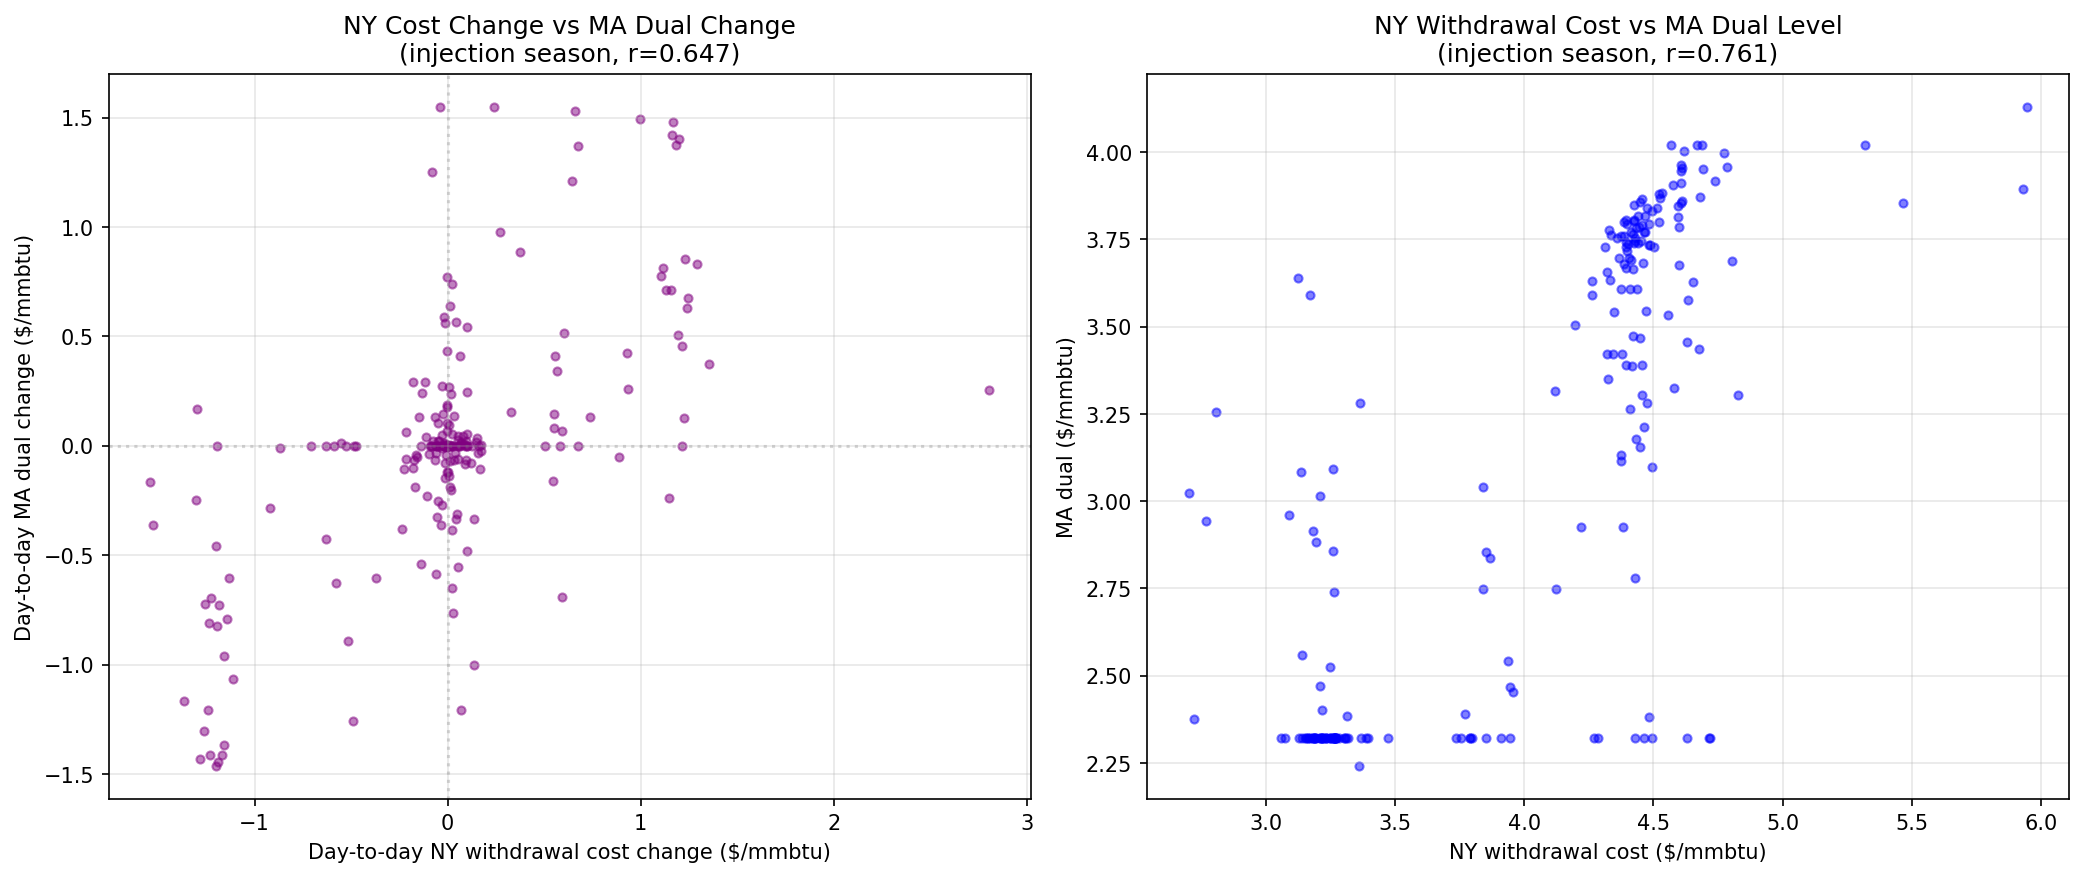
\includegraphics[width=0.88\linewidth]{06_cost_vs_dual_scatter.png}
  \end{figure}
  \vspace{-0.5em}
  {\small \textbf{Left}: Day-to-day changes in NY withdrawal cost vs.\ MA dual ($r = 0.647$). \textbf{Right}: NY withdrawal cost level vs.\ MA dual level ($r = 0.761$). Floor days cluster at bottom-left (low cost $\to$ low dual).}
\end{frame}

% ---- Slide 16: Summary Decomposition ----
\begin{frame}{Summary: Four Mechanisms Decomposed}
  \begin{figure}
    \centering
    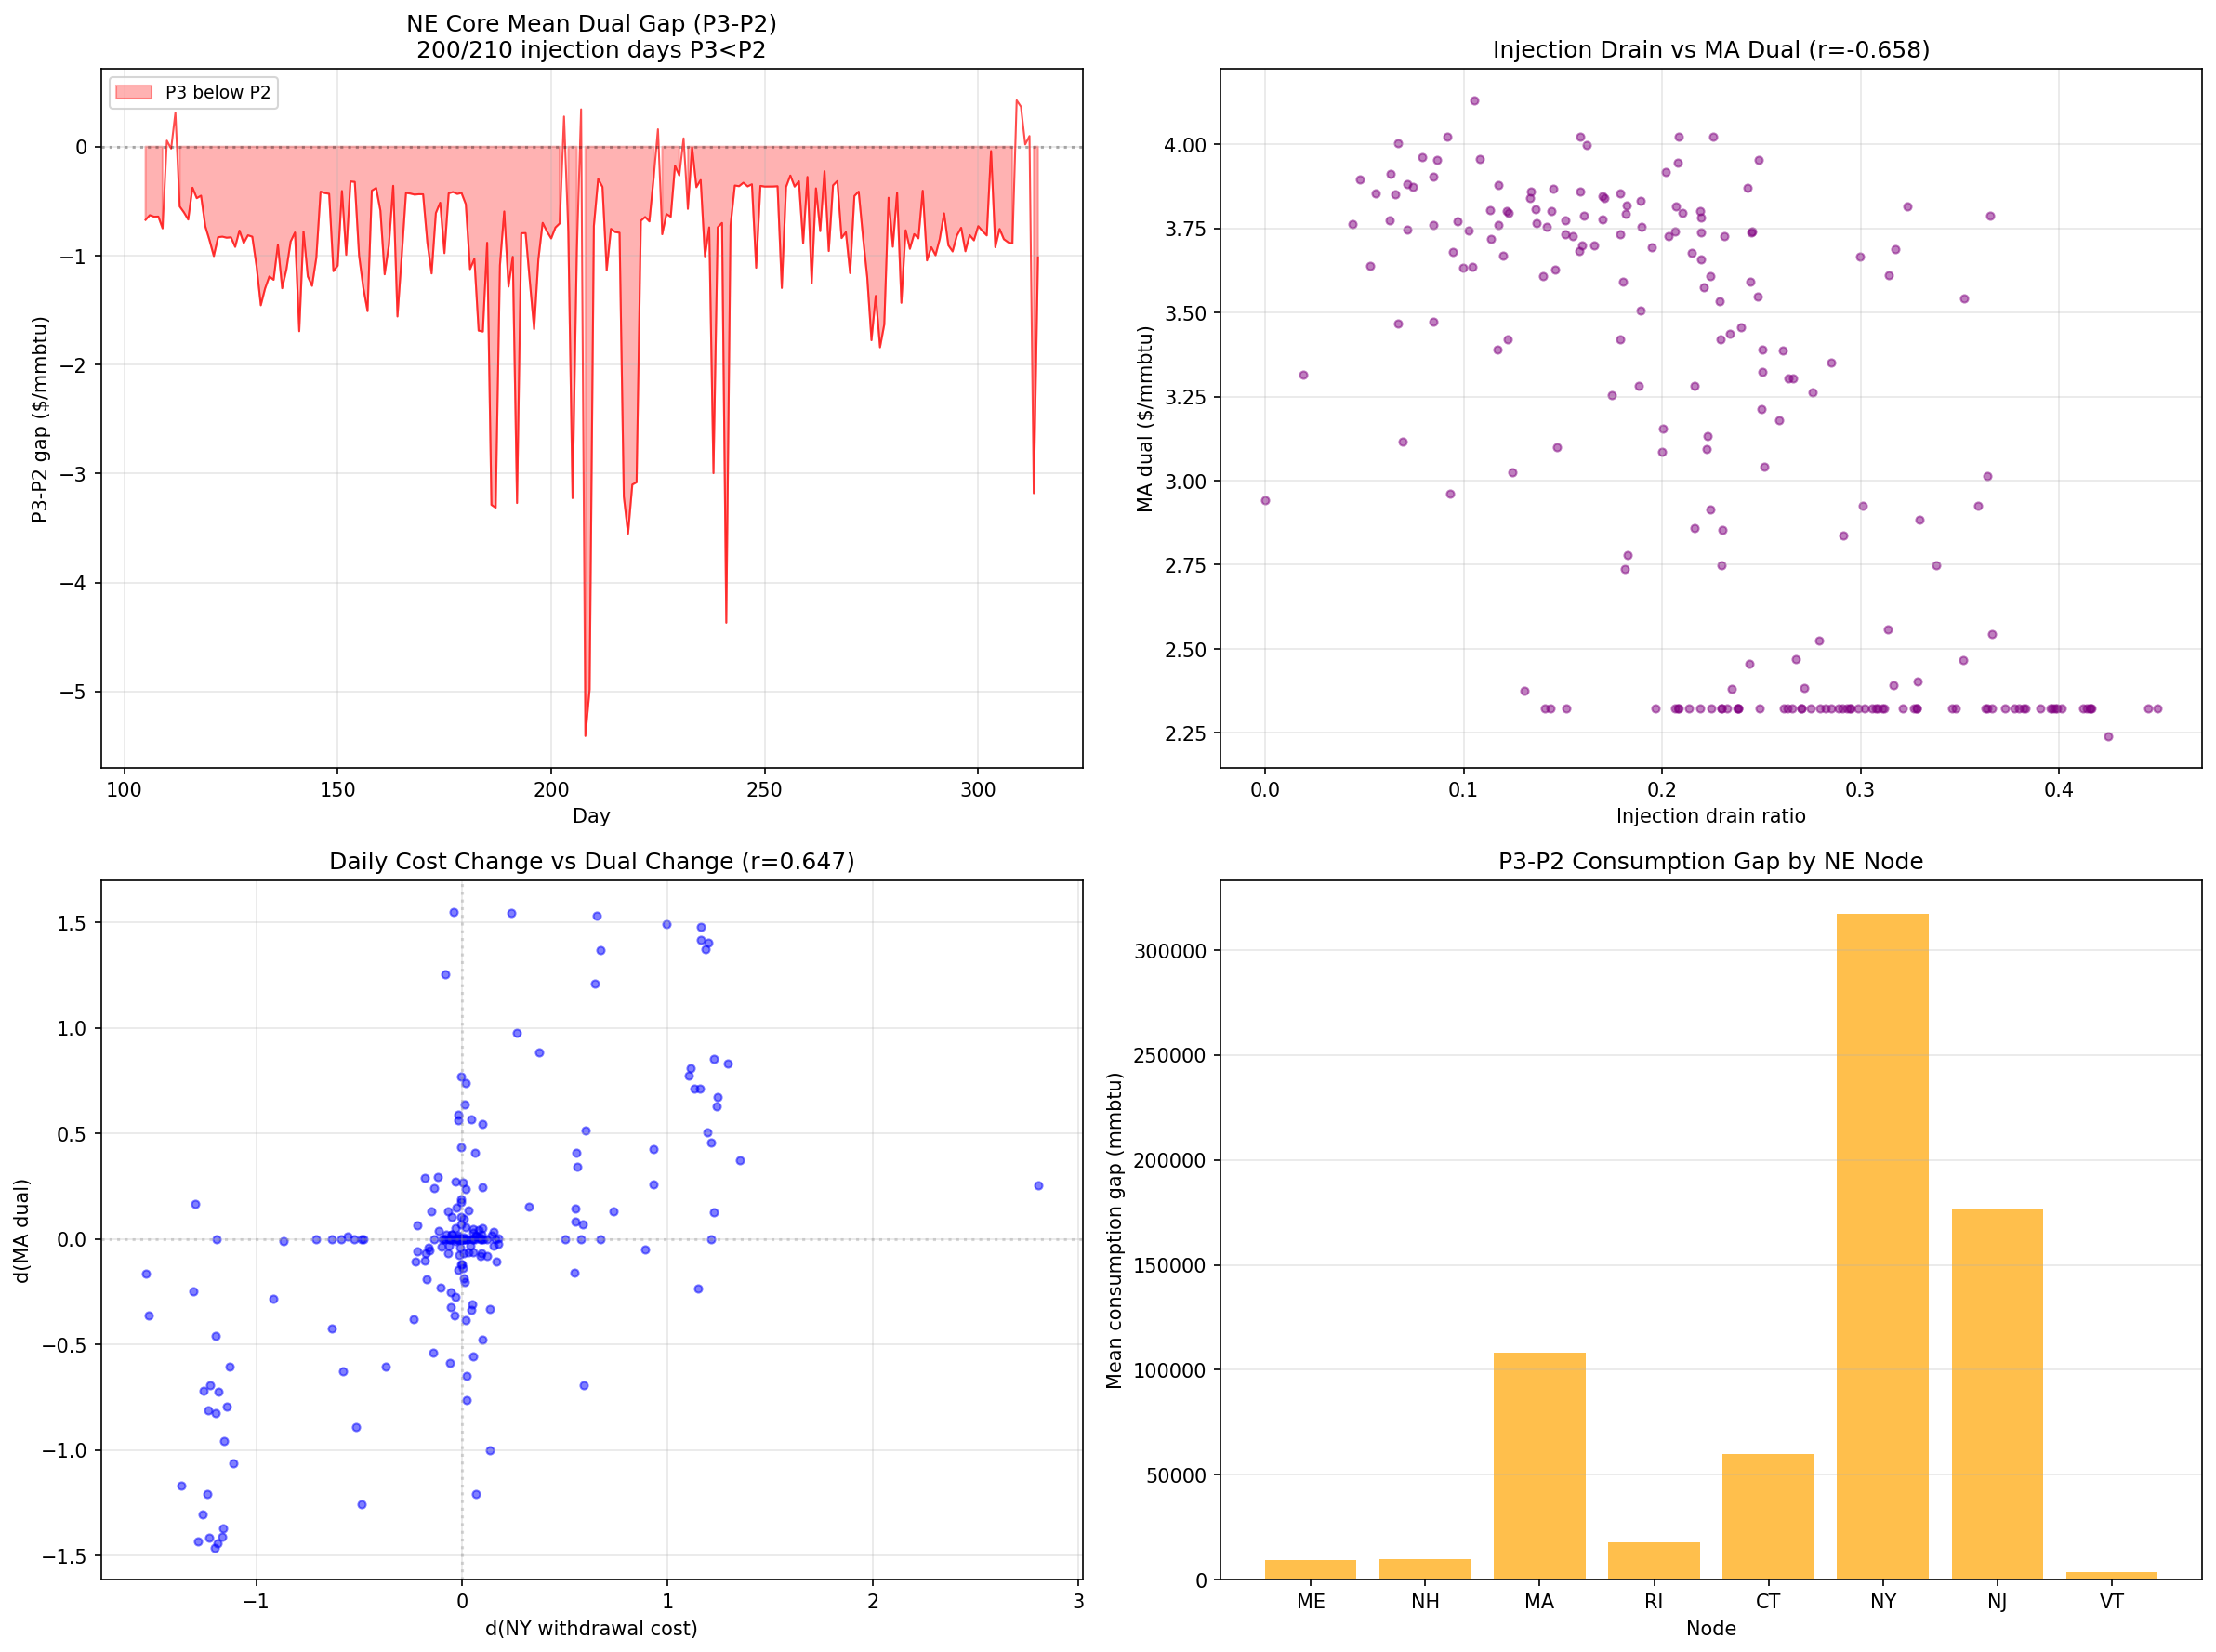
\includegraphics[width=0.82\linewidth]{09_summary_overview.png}
  \end{figure}
  \vspace{-0.5em}
  {\small \textbf{Top-left}: P3$-$P2 gap, P3 below P2 on 200/210 injection days.
  \textbf{Top-right}: Injection drain ratio vs.\ MA dual ($r = -0.66$).
  \textbf{Bottom-left}: Cost change vs.\ dual change ($r = 0.65$).
  \textbf{Bottom-right}: Consumption gap by NE node (NY largest).}
\end{frame}

% ---- Slide 17: MA Floor ----
\begin{frame}{The MA Floor Value}
  On \textbf{65 of 210} injection-season days, MA dual locks to a constant:
  \vspace{0.3em}

  \begin{center}
    {\Large \alert{\$2.322/mmbtu}}
  \end{center}

  \vspace{0.3em}
  \textbf{What happens on floor days}:
  \begin{itemize}
    \item All inbound pipeline flows to MA $= 0$ (completely isolated)
    \item MA price set entirely by local marginal cost (no pipeline arbitrage)
    \item Upstream congestion + injection drain prevent gas from reaching MA
    \item NY storage injection absorbs pipeline capacity that would otherwise serve MA
  \end{itemize}

  \vspace{0.3em}
  \textbf{Mean P3$-$P2 gap during injection season}: \alert{$-$\$0.90/mmbtu} across NE core states.
\end{frame}

%% ============================================================
%% PART IV: RECOMMENDATIONS
%% ============================================================

\section{Recommendations}

% ---- Slide 18: Ranked Fixes ----
\begin{frame}{Recommended Fixes (Ranked)}
  \begin{enumerate}
    \item \textbf{Relax \texttt{RegionInjectionPct}} ($=$ $\to$ $\leq$) \\
      {\small Target: forced injection drain. Risk: \textcolor{okgreen}{Low} --- only affects Part 3 injection allocation.}
    \vspace{0.4em}
    \item \textbf{Relax \texttt{TotalDailyInjection}} ($=$ $\to$ $\leq$) \\
      {\small Target: injection drain + congestion. Risk: \textcolor{orange}{Medium} --- may cause storage to undershoot targets.}
    \vspace{0.4em}
    \item \textbf{Smooth the rolling storage price window} \\
      {\small Target: withdrawal cost volatility. Risk: \textcolor{okgreen}{Low} --- only changes price calculation.}
    \vspace{0.4em}
    \item \textbf{Check PA $\to$ NY pipeline capacity data} \\
      {\small Target: congestion bottleneck. Risk: \textcolor{orange}{Medium} --- only appropriate if current data is incorrect.}
  \end{enumerate}
\end{frame}

% ---- Slide 19: Next Steps ----
\begin{frame}{Next Steps}
  \begin{enumerate}
    \item \textbf{Run relaxed injection model} \\
      {\small Modified model files ready (\texttt{v14\_gas\_model\_dev\_relax\_inject.py}, \\\texttt{v14\_gas\_model\_dev\_relax\_both.py}). Need 372-day run to validate.}
    \vspace{0.4em}
    \item \textbf{Propagate \texttt{Qstep\_prod} fix to production} \\
      {\small Dev $\to$ \texttt{v14\_model\_run\_files\_base/}. Confirmed: 0\% production change, safe to merge.}
    \vspace{0.4em}
    \item \textbf{Recalibrate with corrected model} \\
      {\small Re-run grid search over production/QPS/storage parameters with the fix applied.}
    \vspace{0.4em}
    \item \textbf{Validate against NGI prices} \\
      {\small Compare corrected duals to observed hub prices; compute distance metrics.}
  \end{enumerate}

  \vspace{0.5em}
  \begin{block}{Status}
    Investigation 1 (\textcolor{okgreen}{resolved}): \texttt{Qstep\_prod} $=$ $\to$ $\leq$. \\
    Investigation 2 (\textcolor{orange}{in progress}): NE injection season --- fix candidates identified, awaiting runs.
  \end{block}
\end{frame}

\end{document}
